%%%%
\section{África}

A poluição do ar ambiental nas cidades dos países em desenvolvimento
guarda algumas similaridades com as cidades dos países desenvolvidos, já que 
ambas possuem algumas fontes poluidoras que são características de meios urbanos, 
tais como, tráfego de veículos automotivos, indústrias, geração de 
eletricidade por usina hidrelétrica ou termoelétrica, entre outras. 

No entanto, em cidades de países de industrialização tardia, soma-se a esta 
poluição, comum a meios urbanos, agravantes decorrentes a incapacidade do 
Estado em atender toda a população nas demandas urbanas de infraestrutura, 
como por exemplo, no provimento da energia necessária para realização de 
atividades cotidianas, tais como, transporte, iluminação ou alimentação. 
As alternativas comuns encontradas pela população destas cidades são: queima da 
biomassa para cozimento de alimentos, uso de querosene para iluminação 
noturna e contínuo uso de frota veicular com tecnologias ultrapassadas
\citep{brauer2012}.

Esses fatores citados acima e a urbanização rápida e descontrolada ocorrida na
última década fazem com que cidades da Ásia, África e Oriente 
Médio possuam os maiores níveis de poluição do ar ambiental do mundo 
\citep{brauer2012}.

Em 2015, a África contava com $1.186,178$ habitantes, ficando atrás 
apenas da Ásia, que possuía $4.393,296$ habitantes no mesmo ano. 
A África é o terceiro maior continente em extensão, com área territorial 
de 30 milhões de quilômetros quadrados, abrigando 54 países independentes 
\citep{UN}.

Existe uma barreira natural formada pelo \textbf{Deserto do Saara}
separando norte e sul da África. Separação não só geográfica, como
social, étnica e econômica. 

A África Subsariana \textbf{(SSA)}, localizada ao sul do 
\textbf{Deserto do Saara}, conta com os países maios pobres do mundo, mas que 
nas últimas décadas iniciaram um processo intenso de urbanização \citep{UN}. 
   	
%%%%
\subsection{África Subsariana \textbf{(SSA)}}

A África Subsariana \textbf{(SSA)} é atualmente a região no mundo com a maior 
taxa de transição da população rural - ainda predominante - para cidade
\citep{MONTGOMERY2008}. 

Até 2003, nenhuma cidade da \textbf{SSA} possuía sistemas de monitoramento 
sistemático de poluição do ar, somente medidas esporádicas realizadas
por universidades, mas que revelaram concentrações de poluentes altíssimas e 
acimas dos recomendados pela Organização Mundial de Saúde \textbf{OMS},
fato esse que levou pesquisadores do mundo inteiro a 
realizarem estudo ambientais no continente \citep{EZZATI2004}. 
Segundo \cite{aboh2009} ainda há pouco estudos de aerossol atmosférico 
em países africanos, mas o interesse da comunidade acadêmica cresceu
nos último anos.
 
O aerossol atmosférico africano também desperta interesse, pois afeta o clima 
(radiação, umidade, vento, etc) do mundo.

Diferente dos países industrializados, onde as principais fontes de poluição 
são os setores da industria e do transporte, nos países da \textbf{SSA} a 
queima de biomassa assume a primazia, sendo comum o seu uso no cozimento 
de alimentos, tanto em regiões urbanas quanto rurais \citep{SMITH2004}. 

Estas são algumas características regionais da \textbf{SSA} que ampliam as 
diferenças do perfil de fontes poluidoras do ar comparada com cidades 
de países desenvolvidos: população predominantemente rural,
vias não pavimentadas, altas taxa de crescimento populacional, população jovem,
inexistência de sistemas de monitoramento sistemático em larga escala do meio 
ambiente, queima de biomassa em residências e comércio para o preparação
de alimentos, entre outros. 

%%%%
\subsection{Gana}

Gana situa-se no continente africano, 5 graus a norte do Equador e 
faz fronteira com a Costa do Marfim a oeste, ao norte com Burkina
e a leste com Togo. 

Com clima equatorial, possui praticamente duas estações climáticas:

\begin{itemize}
  \item estação seca, caracterizada pelo ar seco e pela poeira do harmatão. 
       Começa no meados de Novembro se estende até metade de Março.
 \item estação chuvosa, começa em Abril e acaba em outubro, tendo maior
       intensidade entre Abril e Julho.
\end{itemize}

Um vento quente e seco provindo de nordeste sopra entre Novembro e Fevereiro 
e é chamado de Harmatão. O Harmatão vem carregado de poeira do 
\textbf{Deserto do Saara} e é a maior fonte de poeira do mundo
\citep{breuning2005}.

O \textbf{United States Department of Commerce National Oceanic 
and Atmospheric (NOAA)} mantém um banco de dados com parâmetros 
meteorológicos do mundo inteiro enviado por estações meteorológicas 
cadastradas \citep{noaa}. 

Para avaliação do perfil dos parâmetros meteorológicos locais
utilizou-se dados horários de Setembro de 2006 à Junho de 2008 
coletados na estação meteorológica do aeroporto de Acra 
(\textbf{Kotoka International Airport}) cadastrado na \textbf{NOAA}.

Plotando-se o gráfico da figura \ref{fg:rosaCompleta}, 
que mostra a distribuição de frequência de direção dos ventos bem como a 
intensidade, verifica-se que a direção predominante de origem dos ventos 
é sudoeste. 

\begin{figure}[H]
  \centering
  \includegraphics[width=0.5\textwidth]{../outputs/windRoseNoaaHarvard.pdf}
  \caption{Rosa do ventos entre
           Setembro de 2006 e Junho de 2008. Utilizou-se dados 
           do \textbf{Kotoka International Airport} de Acra 
           \label{fg:rosaCompleta}}
\end{figure}

No gráfico da figura \ref{fg:rosaCompleta} a observação horária da direção e 
intensidade dos ventos, identifica-se um regime de brisa marinha bem 
definido, com ventos de sul quando sol a pino, mas se deslocando a oeste com a 
entrada da noite. 

No gráfico de rosa dos ventos mensal \ref{fig:windRose_mensal} nota-se 
perceptível diferença entre os dois períodos climáticos, 
pois no Verão temos maior quantidade de radiação solar, fortalecendo a 
formação de brisa marinha e, consequentemente, deslocando mais para o 
oeste a distribuição de frequência nas direções dos ventos.

\begin{figure}[H]
  \centering
  \includegraphics[width=1\textwidth]{../outputs/windRose_horaria.pdf}
  \caption{ \citep{carslaw2012} \label{fig:windRose_horaria}}
\end{figure}

\begin{figure}[H]
  \centering
  \includegraphics[width=1\textwidth]{../outputs/windRose_mensal.pdf}
  \caption{ \citep{carslaw2012} \label{fig:windRose_mensal}}
\end{figure}

Nos meses de ocorrência do Harmatão (inverno), não há aumento siginicativo 
na frequência de ventos de nordeste, pois o vento do Harmatão passa por Gana 
em altas altitudes, não influenciando os ventos locais \citep{breuning2005}. 

Os últimos dois censos demográficos realizados em Gana datam
de 2000 \citep{ghanacensus2003} e 2010 \citep{ghanacensus2013}. Os
dados resultantes podem ser encontrados no portal de dados abertos
do Governo Federal de Gana \citep{opendataghana}.

A população de Gana em 2000, $18,9$ milhões de habitantes, subiu para $24,7$ 
milhões em 2010, aumento de $30\%$ no intervalo dos dois censos demográficos.

Segundo censo demográfico de 2010, $49\%$ da população está no meio rural e 
$61\%$ no meio urbano, sendo que as mulheres representam $51,2\%$ da polulação
total.

A pirâmede etâria de Gana, figura \ref{fig:piramedegana}, indica população 
jovem e expectativa média de vida não muito maior que 50 anos. 

\begin{figure}[H]
  \centering
  \includegraphics[width=0.5\textwidth]{../outputs/piramide_etaria.pdf}
  \caption{Pirâmide etária Gana plotada com dados do censo 
           demográfico de 2010 \citep{ghanacensus2013} \label{fig:piramedegana}}
\end{figure}

A economia de Gana, antes essencialmente dominada pela agricultura, 
agora está distribuída entre: industria $19\%$, agricultura $30\%$ 
e serviços $51\%$ \citep{ghanacensus2013}.

Na industria, recebe destaque fabricação e exportação de aparelhos digitais, 
automóveis e navios. Em termos de matéria primária, há siginicativa 
exportação de hidrocarbonetos e minerais \citep{ghanacensus2013}.

O produto interno bruto (PIB) per capita anual de Gana em 2010 foi
de \$ 1.323,09 USD e no Brasil no mesmo ano \$ 11.124,09 USD.
O gráfico da figura \ref{fg:pib} apresenta o \textbf{PIB} de Gana e do Brasil 
calculado pelo Banco Mundial \citep{bancomundial}.

\begin{figure}[H]
\begin{center}
  \includegraphics[width=0.5\textwidth]{../outputs/PIBGhanaBrazil.pdf}
  \caption{\textbf{PIB} do Brasil e de Gana. Plotado com dados do 
           Banco Mundial \citep{bancomundial} \label{fg:pib}}
\end{center}
\end{figure}

A responsabilidade do controle, fiscalização e monitoramento das 
atividades poluídoras em Gana é realizado pela 
\textbf{Ghana Environmental Protection Agency (EPA Ghana)}, que é 
hierarquicamente subordinada ao 
\textbf{Ministério de Meio Ambiente, Ciência, Tecnologia e Inovação} do 
Governo Federal de Gana.

%%%%
\subsection{Região Metropolitana de Acra \textbf{(RMA)}}

Acra é uma cidade litorânea e é a capital de Gana. Está localizada 
no Golfo Guiné tendo área total de mais de  $2500 km^2$, com elevações que 
variam de 0 até 60 metros do nível do mar \citep{ARKU2008}.

A Região Metropolitana de Acra \textbf{(RMA)} agrega outras 9 cidades
além de Acra e conta com uma população total de 4 milhões de habitantes (2010). 
Com economia baseada majoritariamente na industria e em serviços, 
$90,5\%$ da polulação está alocada em área urbana \citep{ghanacensus2013}.

Em 2010, havia aproximadamente 1000 fazendas urbanas com produção de vegetais e
frutas para consumo local de Acra. Em geral, as irrigações nessas plantações
são feitas por água não tratada, provinda de córregos locais. 
Altos indíces de metais pesados (Fe, Mn, Cu, Zn, Pb, Ni, Cr, Cd, Co)
são encontrados nos alimentos produzidos nessas fazendas, pois resíduos de
residências são despejados diretamanente nos nesses córregos \citep{lente2014}.

A densidade populacional em \textbf{(RMA)} é de 1205 $habitantes/km^2$, 
enquanto que na Região Metropolitana de São Paulo \textbf{(RMSP)} é de 
2476 $habitantes/km^2$ \citep{ibge2011}. 

\textbf{Driver and Vehicle Licensing Authority (DVLA)} é o
departamento do governo de Gana que cuida dos registros de automóveis
e em 2009 Gana contava com 1,12 milhões de veículos legais. 
A tabela \ref{table:dvla} mostra que a frota dobrou em um década.
Ressalta-se que além dos veículos legalizados, Gana conta com uma frota grande
de veículos envelhecidos e não são registrados, mas circulantes. 

\begin{table}[H]
 \centering
  \begin{tabular}{rr}
  \hline
  Ano & Veículos Registrados \\ 
  \hline
  2000 & 511.083 \\ 
  2001 & 567.780 \\ 
  2002 & 613.153 \\ 
  2003 & 643.824 \\ 
  2004 & 703.372 \\ 
  2005 & 767.067 \\ 
  2006 & 841.314 \\ 
  2007 & 841.314 \\ 
  2008 & 1.033.140 \\ 
  2009 & 1.128.138 \\ 
  \hline
  \end{tabular}
  \caption{Frota veícular de Gana \citep{dvla} \label{table:dvla}}
\end{table}

Segundo a EPA-GH \citep{epa2015} as fontes de poluição do ar ambiental 
majoritárias em Acra são:

\begin{itemize}
 \item Emissões veiculares, principalmente emissões de veículos antigos sem 
       manutenção;
 \item Emissões industriais;
 \item Queima de lixo e outros materiais a céu aberto;
 \item Poeira de ressupensão de solo, pois há muitas vias ainda não pavimentadas;
 \item Poeira carregada por vento seco do \textbf{Deserto do Saara}, o Harmatão.
\end{itemize}

Acra é mundialmente conhecida por receber ilegalmente lixo 
eletrônico dos países desenvolvidos, que são então derretidos, de forma
imprópria, para obtenção de cobre pela população local. 
O depósito de lixo eletrônico, conhecido como \textbf{e-waste}, 
fica no bairro \textbf{Agbogbloshie}, $4 km$ a sudoeste de \textbf{Nima}
\citep{asampong2015}.

\begin{figure}[H]
  \centering
  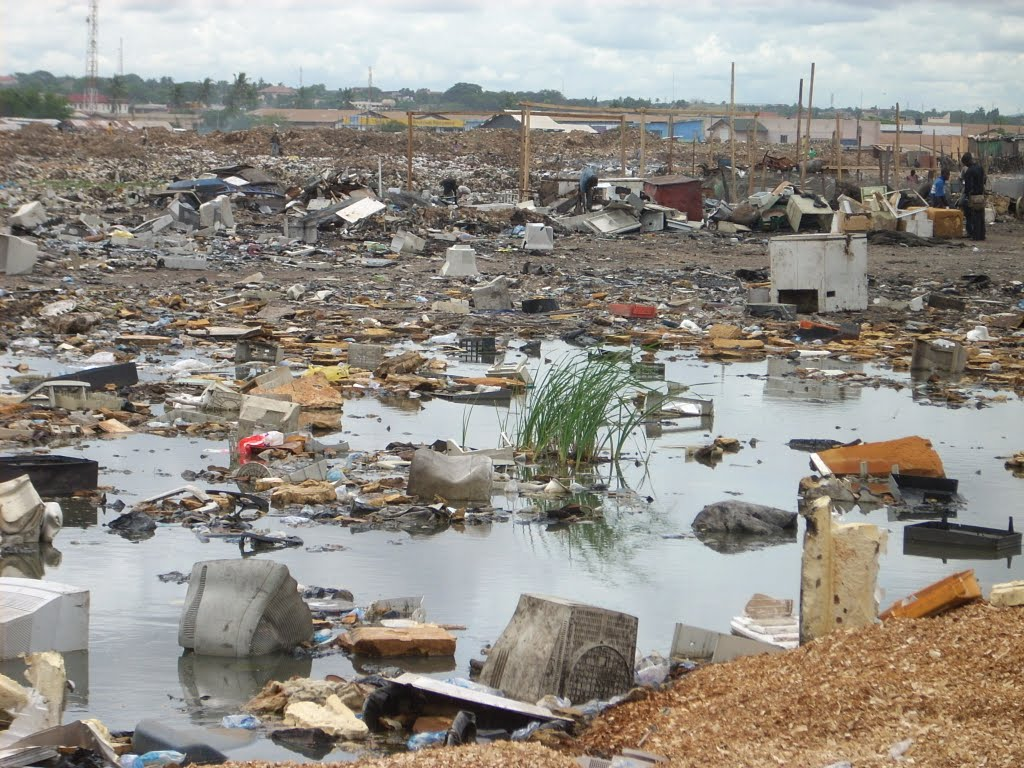
\includegraphics[width=0.5\textwidth]{../inputs/images/ewaste_jack_caravano.jpg}
  \caption{Foto do bairro de Agbogbloshie em Acra. Autorizado por Jack Caravanos, 
           Professor da \textbf{School of Public Health} em \textbf{Hunter College, CUNY}
           Nova Iorque, Estado Unidos da América. \label{fig:ewaste}}
\end{figure}

%%%%
\subsection{Nima}

Nima é um dos bairros mais pobres de Acra e formada de assentamentos não 
planejados compostos principalmente de migrantes das partes rurais e 
imigrantes de países vizinhos que buscam oportunidades de empregos na capital. 
Com moradias extremamentes improvisadas, carece de sistema tratamento de esgoto, 
fornecimento de água potável e eletricidade. 

É conhecida localmente por uma feira de comidas típicas permanentemente 
instalada na região (\textbf{Nima Market}), que é inclusive visitada por turistas.
Com população de origem de diversas partes de Gana, Nima possui 
alta diversidade cultural e religiosa.

O principal meio de transporte dos trabalhadores de Nima para a zona industrial
e de serviços de Acra é feito por vans. 
Muitas vias não são pavimentadas e a intensa movimentação de veículos causa 
levantamento de poeira do solo.

O carvão e a lenha são as principais fontes de energia para preparação de 
alimentos e foto da figura \ref{fig:nima} há imagens mostrando como as cozinhas
são equipadas. 

\begin{figure}[H]
  \centering
    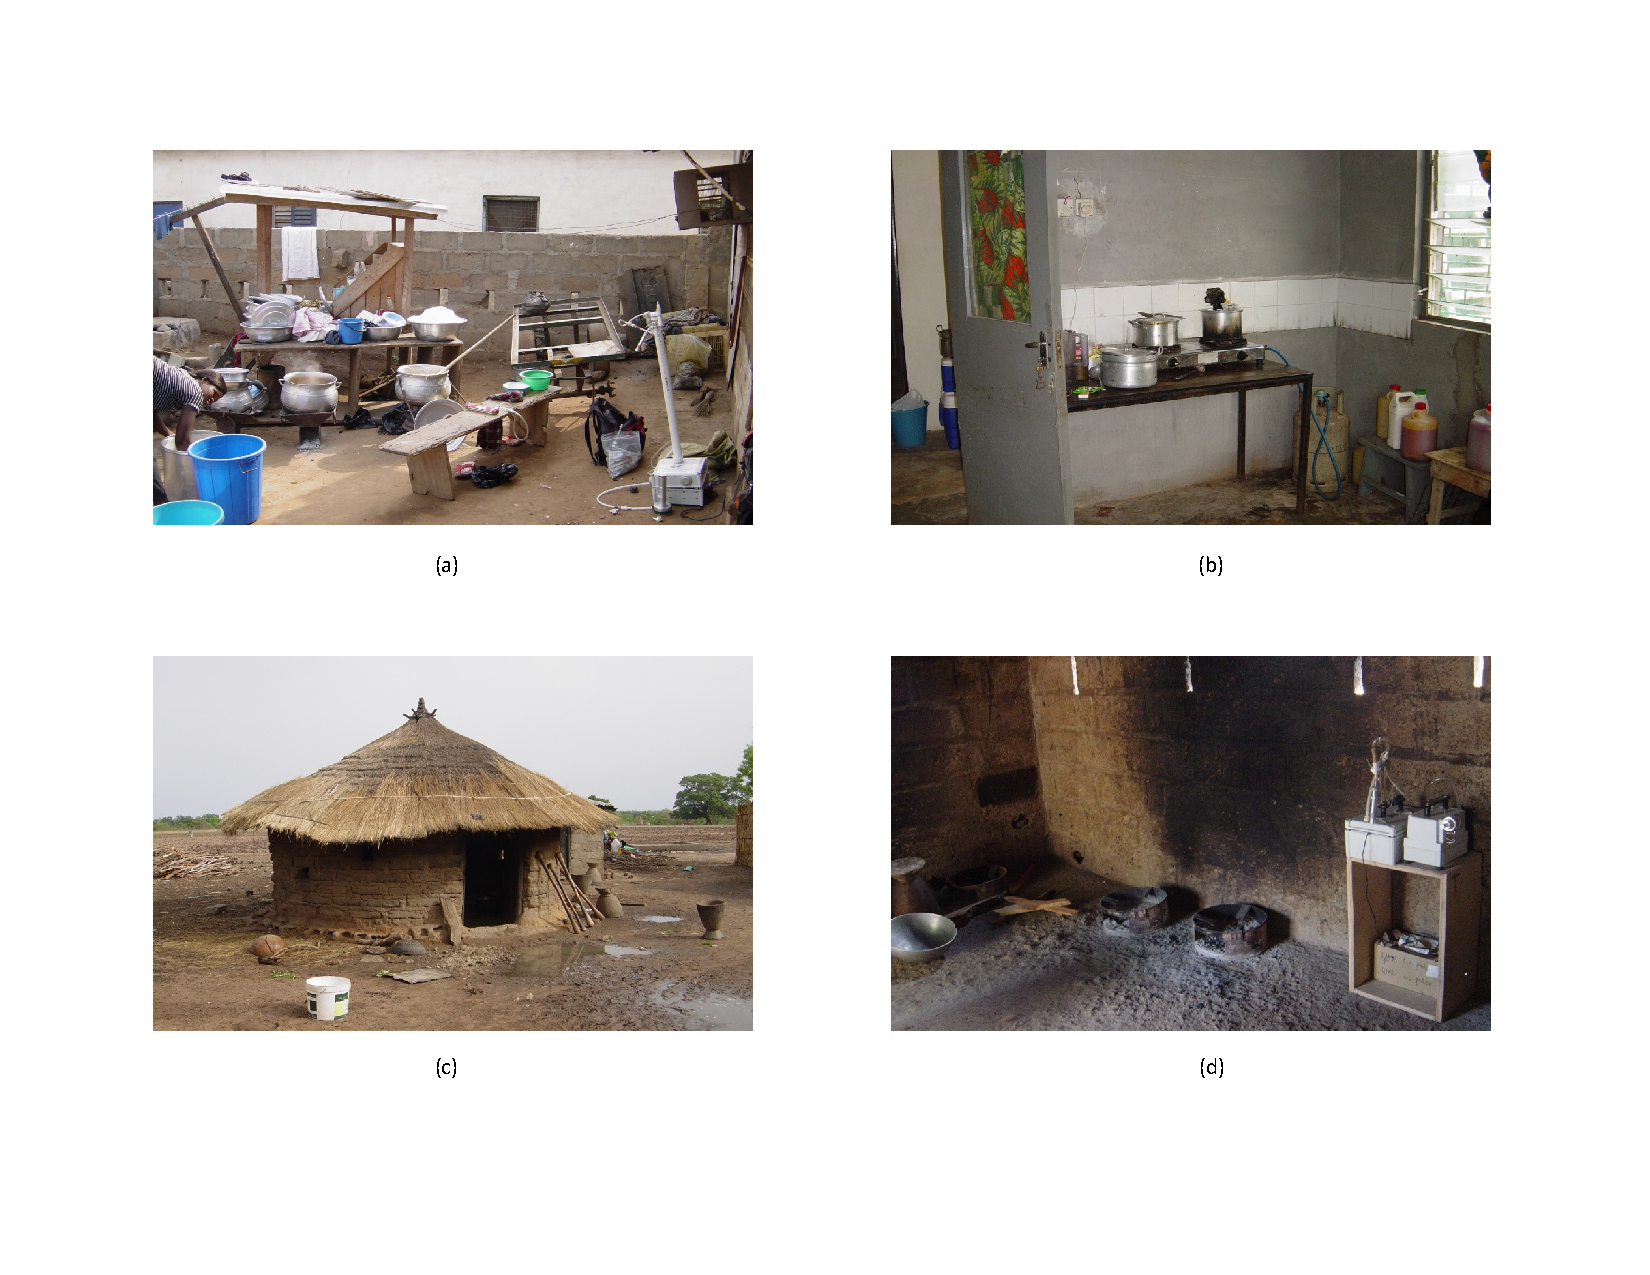
\includegraphics[width=0.7\textwidth]{../inputs/images/zheng/nima.pdf}
    \caption{Fotos de residências de Nima, por Raphael Arku \label{fig:nima}}
\end{figure}
